\subsection{Zusammenfassung Skinning}

Skinning verfolgt das Ziel das sich das Modell natürlich bei jeder Bewegung vom Skelett mit bewegt. Dies wird durch viele Faktoren beeinflusst. Wie zum Beispiel dem Material der Figur oder den physikalischen Gesetzmäßigkeiten des Films. Es gibt viele Ansätze, die vom Einsatz komplexer Hardware reichen um physiologisch komplizierte Prozesse wie das Atmen darzustellen bis hin zu einfachen geometrischen Ansätzen. 

Diese basieren auf der Grundlage die Transformationen nach physiologischen Eigenschaften zu modifizieren. Das primäre Beispiel hierfür ist wohl die Vergabe von Gewichten an einzelne Punkte auf der Haut um die Abhängigkeit von mehreren Knochen zu simulieren. 

Ich Bereich des geometrischen Skinning ist Linear Blend Skinning der Standart auf Grund seiner Einfachheit und Performanz. Dieser hat allerdings das Problem durch Volumenverlust Artefakte zu erzeugen. Dual Quaternionen Blend Skinning behebt dies bei vergleichbarer Rechenleistung. Allerdings erzeugt auch dieser bei manchen Rotationen Artefakte und erlaubt keine Volumenveränderungen. Die beiden Verfahren nochmal im Vergleich bei unterschiedlicher Gewichtsverteilung in (Abbildung).

\begin{figure}[t]
	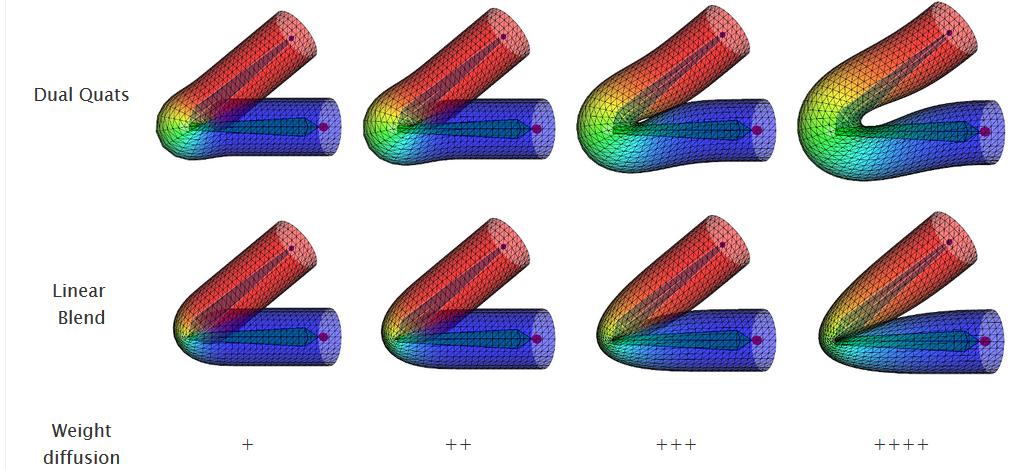
\includegraphics[width=13cm]{01_Skinning/pics/lbsvsdqs.png}
	\caption[Geometrisches Skinning im Vergleich]{Die erste Reihe zeigt Dual Quaternion Blend Skinning, die zweite Linear Blend Skinning. Die letzte Reihe bestellt die Gewichtsverteilung in jeder Spalte. Entnommen von}
	\label{weights_fig1}
\end{figure}